\documentclass[12pt,a4paper,twoside,openright,headsepline,footsepline]{scrreprt}

\usepackage[top=1.5cm,bottom=1.5cm,footskip=.8cm,footnotesep=1cm,includeheadfoot]{geometry}

\usepackage[ngerman]{babel}

\usepackage[utf8]{inputenc}

\usepackage{scrpage2}
\pagestyle{useheadings}

\usepackage[pdftex]{graphicx}
\usepackage{epstopdf}


\usepackage{cite}

\usepackage{amsmath}
\usepackage{amssymb}

\usepackage{amsthm}
\theoremstyle{definition}
\newtheorem*{ziel}{Zielsetzung}
\newtheorem{defi}{Definition}[section]
\newtheorem*{fazit}{Fazit}

\usepackage{dsfont}
\newcommand{\R}{\mathds{R}}
\renewcommand{\d}{\mathrm{d}}

\usepackage{siunitx}

\sloppy


\usepackage{hyperref}


\begin{document}
\begin{frontmatter}
  \title{Curvature approximation on surfaces -- A Discrete Exterior Calculus Approach}

  \author{I.~Nitschke\fnref{fn1}}
  \ead{ingo.nitschke@tu-dresden.de}
  
  \author{A.~Voigt\fnref{fn1,fn2}}
  \ead{axel.voigt@tu-dresden.de}

  \fntext[fn1]{Department of Mathematics, TU Dresden, 01062 Dresden, Germany}
  \fntext[fn2]{Center of Advanced Modeling and Simulation, TU Dresden, 01062 Dresden, Germany}

  \begin{abstract}
    Lorem ipsum dolor sit amet, consetetur sadipscing elitr, sed diam nonumy eirmod tempor invidunt ut labore et dolore magna aliquyam erat, sed diam voluptua. At vero eos et accusam et justo duo dolores et ea rebum. Stet clita kasd gubergren, no sea takimata sanctus est Lorem ipsum dolor sit amet. Lorem ipsum dolor sit amet, consetetur sadipscing elitr, sed diam nonumy eirmod tempor invidunt ut labore et dolore magna aliquyam erat, sed diam voluptua. At vero eos et accusam et justo duo dolores et ea rebum. Stet clita kasd gubergren, no sea takimata sanctus est Lorem ipsum dolor sit amet. Lorem ipsum dolor sit amet, consetetur sadipscing elitr, sed diam nonumy eirmod tempor invidunt ut labore et dolore magna aliquyam erat, sed diam voluptua. At vero eos et accusam et justo duo dolores et ea rebum. Stet clita kasd gubergren, no sea takimata sanctus est Lorem ipsum dolor sit amet.
  \end{abstract}

  \begin{keyword}
    Surfaces \sep Curvature \sep DEC
  \end{keyword}
\end{frontmatter}

\section{Introduction}
Lorem ipsum dolor sit amet, consetetur sadipscing elitr, sed diam nonumy eirmod tempor invidunt ut labore et dolore magna aliquyam erat, sed diam voluptua. At vero eos et accusam et justo duo dolores et ea rebum. Stet clita kasd gubergren, no sea takimata sanctus est Lorem ipsum dolor sit amet. Lorem ipsum dolor sit amet, consetetur sadipscing elitr, sed diam nonumy eirmod tempor invidunt ut labore et dolore magna aliquyam erat, sed diam voluptua. At vero eos et accusam et justo duo dolores et ea rebum. Stet clita kasd gubergren, no sea takimata sanctus est Lorem ipsum dolor sit amet. Lorem ipsum dolor sit amet, consetetur sadipscing elitr, sed diam nonumy eirmod tempor invidunt ut labore et dolore magna aliquyam erat, sed diam voluptua. At vero eos et accusam et justo duo dolores et ea rebum. Stet clita kasd gubergren, no sea takimata sanctus est Lorem ipsum dolor sit amet.


\section{Discrete Exterior Calculus (DEC)}
  The Discrete Exterior Calculus \citep{hirani, desbrun} defines discrete differential \mh{p}{forms} on a triangulated mesh (simplicial complex).
  For surface meshes, i.e. triangulated orientable \mh{2}{manifolds}, the degree of the discrete \mh{p}{forms} is 0, 1 or 2
  and their are represented by scalars on vertices, edges, triangles or chains of them. 
  Operators for the differential forms, like the exterior derivation \( \exd \) or the hodge star \( \star \), can be approximated by expressions on the discrete
  geometrical structure. 
  E.g. the integral over a triangle of the exterior derivation \( \exd \) for a \mh{1}{form} can be expressed as the integral of the
  \mh{1}{form} over the boundaries edges of the triangle. 
  This follows directly from the Stokes Theorem \citep[Ch. 7]{marsden}. 
 
  \subsection{Discrete manifolds}
    In our setting, the surface meshes are linear triangulations of orientable closed \mh{2}{manifolds}.
    Such a Triangulation are sets of \mh{p}{simplices} \( \left\{ \sigma^{p} \right\} \) of the same degree \( p \), e.g. sets of vertices,
    edges and triangles, and form a simplicial complex of dimension \( n=2 \).
    A simplicial complex \( K \) comply two essential rules:
    \begin{enumerate}
      \item Every face of a simplex \( \sigma^{p}\in K \) is in \( K \).
      \item The intersection of two simplices in \( K \) is either in \( K \) or empty.
    \end{enumerate}
    We shortly write \( \sigma^{q}\prec\sigma^{p} \) (or \( \sigma^{p}\succ\sigma^{q}) \)), 
    iff \( q<p \) and \( \sigma^{q} \) is a face of \( \sigma^{p} \). 
    It is required, that the polytop
    \begin{align}
      |K| &:= \bigcup_{\sigma\in K} \sigma 
    \end{align}
    of \( K \) is a \mh{C^{0}}{manifold} and we call \( K \) a manifold-like simplicial complex.
    For a higher consistence to the smooth model, we assume that the simplicial complex is orientable,
    i.e. all triangles \( \sigma^{2}\in K \) have the same orientation.
    The orientation of a triangle is define as one of the two equivalence classes, that arise from the kind of counting the vertices
    (clockwise or counterclockwise).
    We write \( \sigma^{2}=\left[ v_{0}, v_{1}, v_{2} \right] \) to mark the order of the vertices \( v_{i} \).
    In the same manner a edge \( \sigma^{1} = \left[ v_{0}, v_{1} \right] \) get an declared orientation.
    Such a manifold-like orientable simplicial complex is called a primal mesh.

    For the existence of a dual mesh, we also need, that the primal mesh is well-centered, 
    i.e. for all triangles \( \sigma^{2}\in K \) the circumcenter \( c(\sigma^{2}) \) lies in the interior of \( \sigma^{2} \).
    A dual mesh \( \csd K \) is the circumcenter subdivision of a well-centered primal mesh \( K \).
    For a explanatory example see figure \ref{figExSubdivision}.
    The dual mesh is also a primal mesh, but it is not well-centered.

    \begin{figure}
      \begin{minipage}[htp]{.24\textwidth}
        \centering
        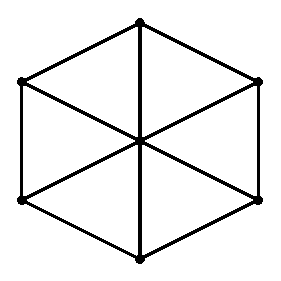
\includegraphics[width=.9\textwidth]{bilder/tikz/K.eps}
      \end{minipage}\hfill
      \begin{minipage}[htp]{.24\textwidth}
        \centering
        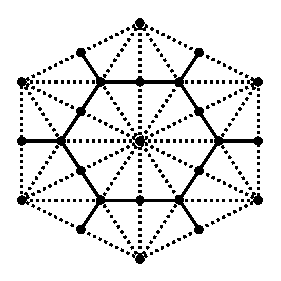
\includegraphics[width=.9\textwidth]{bilder/tikz/CsdK.eps}
      \end{minipage}
      \caption{Example of a circumcenter subdivision.
               Left: A primal mesh \( K \).
               Right: The resultant dual mesh \( \csd K \). 
               All new vertices are the circumcenters of the triangles and edges.
               The solid lines highlights the edges of the Voronoi mesh \( \star K \leq \csd K \).}
      \label{figExSubdivision}
    \end{figure}

    \subsection{Chains}
    An important role in the DEC are chains. 
    A \mh{p}{chain} is the formal sum of \mh{p}{simplices} with coefficients in \( \Z \). 
    Therewith, we denote the space of all \mh{p}{chains} of \( K \)  by
    \begin{align}
      C_{p}(K) &:= \left\{\sum_{\sigma\in K^{(p)}}a_{\sigma}\sigma \middle| a_{\sigma}\in\Z \right\} \formpunkt
    \end{align}
    \( K^{(p)} \) is the set of all \mh{p}{simplices} of \( K \). 
    For chains we can use the universal property, because \( C_{p}(K) \) is a free abelian group with the generating set \( K^{(p)} \).
    Hence, the diagram
    \begin{align}
    \begin{xy}
      \xymatrix{
        C_{p}(K) \ar[rd]^{\widehat{op}} & \\
        K^{(p)} \ar@^{(->}[u] \ar[r]_{op}& \mathfrak{A}
      }
    \end{xy}
  \end{align}
  commutes for a arbitrary abelian group \( \mathfrak{A} \) and homomorphism \( op = \widehat{op}|_{K^{(p)}} \) 
  and \( \widehat{op} \) is unique determinated by \( op \),
  i.e. it is quit enough to define operators for chains only on the simplices. 
  
  \subsection{Geometrical operators}
    The two momentous operators on chains are the boundary operator \( \partial \) and the star operator \( \star \).
    These are the geometrical tools for the discrete exterior derivation \( \d \) resp. the discrete Hodge star \( * \),
    what we will see below.

    \subsubsection{The star operator}
      For a general definition of the star operator \( \star \) see \cite{hirani,desbrun} or \cite[Ch. 7]{siggraphKap7}.
      In our two dimensional well-centered primal mesh case it is enough to define the star operator 
      \( \star: C_{p}(K) \rightarrow C_{2-p}(\csd K) \)
      by 
      \begin{align}
        \label{eqVoronoiCell}
       \star\sigma^{0} &:= \sum_{\sigma^{0} \prec \sigma^{1} \prec \sigma^{2}}
                                                   s_{\sigma^{1} \sigma^{2}} \left[ \sigma^{0}, c(\sigma^{1}), c(\sigma^{2}) \right] \\
       \label{eqVoronoiEdge}
       \star\sigma^{1} &:= \sum_{\sigma^{1} \prec \sigma^{2}}
                                                   s_{\sigma^{2}} \left[ c(\sigma^{1}), c(\sigma^{2}) \right] \\
       \label{eqVoronoiVertex}
       \star\sigma^{2} &:= c(\sigma^{2}) 
      \end{align}
      The factors \( s_{\bullet} \) are signs to prevent orientation properties, like the orientability of the dual mesh.
      \eqref{eqVoronoiCell} describe the Voronoi cell of the primal vertex \( \sigma^{0} \),
      \eqref{eqVoronoiEdge} describe the Voronoi edge of the primal edge \( \sigma^{1} \) (c.p. figure \ref{figExSubdivision})
      and \eqref{eqVoronoiVertex} describe the Voronoi vertex of a primal triangle \( \sigma^{2} \). 
      With the notation \(C_{2-p}( \star K)  \) for the image of \( \star \), 
      the star operator act on \(C_{2-p}( \star K)  \) and map to \( C_{p}(K) \) is for \( p=0,2 \) simply the inverse.
      For \( p=1 \) we must swap the orientation, i.e. \( \star\star\sigma^{1}=-\sigma^{1} \).

    \subsubsection{The boundary operator}
      Let \( K \) be a primal mesh (not necessary well-centered). 
      The boundary operator \( \partial: C_{p}(K) \rightarrow C_{p-1}(K) \) is defined by
      \begin{align}
        \partial\sigma^{p} &:=
                                \begin{cases}
                                  \sum\limits_{i=0}^{p} (-1)^{i} \left[ v_{0}, v_{1}, \ldots, \hat{v}_{i}, \ldots, v_{p} \right] &
                                  \text{for } p=1,2 \\
                                  0 & \text{for } p=0 
                                \end{cases}
      \end{align}
      (\( \hat{v}_{i} \) is omitted) and comply the property \( \partial\circ\partial = 0\).
      This is the authorization to call the sequence \( \left( C_{p}(K), \partial \right) \) (and also \( \left( C_{p}(\star K), \partial \right) \)) 
      \begin{align}
      \begin{xy}
        \xymatrix{
          0 \ar[r] & 
          C_{2}(K) \ar[r]^{\partial} \ar[d]^{\star} & 
          C_{1}(K) \ar[r]^{\partial} \ar[d]^{\star} & 
          C_{0}(K) \ar[r] \ar[d]^{\star} &
          0 \\
          0  & 
          C_{0}(\star K) \ar[l] \ar[u]& 
          C_{1}( \star K) \ar[l]^{\partial} \ar[u] & 
          C_{2}(\star K) \ar[l]^{\partial} \ar[u] &
          0 \ar[l]
        }
      \end{xy}
      \end{align}
      a chain complex.

  \subsection{Discrete differential forms}
    A discrete \mh{p}{form} \( \alpha \) is a homomorphism from the chain group \( C_{p}(K) \) to the additive group \( \R \).
    Thus, the space of discrete \mh{p}{form} is the space of cochains \( \text{Hom}\left( C_{p}(K), \R \right)\), 
    denoted as \( C^{p}(K) \) or, under attention the analogy to smooth differential forms, \( \Omega^{p}_{d}(K) \).
    The crucial map, that define such homomorphisms and give the relation to the smooth forms,
    is the de Rham map
    \begin{align}
    \label{eqDeRham}
      \begin{aligned}
        \psi: \Omega^{p}(M) &\rightarrow C^{p}(L) = \Omega_{d}^{p}(L)\\
                       \alpha   &\mapsto \left( \sigma^{p} \mapsto \int_{\sigma^{p}} \alpha =: \left\langle \psi(\alpha), \sigma^{p} \right\rangle\right)
                       \formpunkt
      \end{aligned}
    \end{align}
    The right hand side is the pairing notation, which we want to use.
    At this, \( L \) is the abstract simplicial complex of \( K \) and arise if all simplices from \( K \) are projected to the underlying
    manifold \( M \), i.e. \( |L| = M  \) and \( L=\pi(K) \) with a projection map \( \pi:|K|\rightarrow M \).
    But the projection and in the most cases the manifold \( M \) is not exactly known, 
    so for interest of simplification we can approximate the integral in \eqref{eqDeRham} with a linear quadrature \( I \) on the vertices of a
    given simplex \( \sigma^{p}\in K \):
    \begin{align}
      \left\langle \psi(\alpha), \pi\left(\sigma^{p}\right) \right\rangle &\approx I_{\sigma^{p}}(\alpha) \formpunkt
    \end{align}
    For \( p=0 \) and a function (\mh{0}{form}) \( f:M\rightarrow\R \) and a vertex (\mh{0}{simplex}) is this exact, 
    i.e.
    \begin{align}
      \left\langle \psi(f), \pi\left(v\right) \right\rangle 
            &= \left\langle \psi(f), v \right\rangle = f(v) \formpunkt
    \end{align}
    For \( p>1 \) the question about evaluating the integral in \eqref{eqDeRham} is pure formal in this paper, 
    because in all of our computation, we can reduce the problems to scalar valued formulations.
    Henceforth, the projection \( \pi \) is omitted in the pairing notation, 
    i.e. we write \( \left\langle \psi(\alpha), \sigma^{p} \right\rangle \) instead of
    \( \left\langle \psi(\alpha), \pi\left(\sigma^{p}\right) \right\rangle \).

  \subsection{DEC operators}
    For the definition of a discrete version of the Hodge star \( * \) or the exterior derivative \( \d \) we can fall back to the
    geometric operators.

    \subsubsection{The discrete Hodge star operator}
      
      
    

\section*{References}
\bibliography{bibl}
\bibliographystyle{elsarticle-harv}

\end{document}
